
%%% Local Variables: 
%%% mode: latex
%%% TeX-master: t
%%% End: 

\chapter{3D播放器设计与实现}
\label{cha:3Dplayerdesignandrealization}

\section{实验平台}
\label{sec:3dplayerhardwareplatform}

\subsection{NVIDIA 3D Vision套装介绍}
\label{subsec:nvidia3dvisionbrief}

% 此处可以插入一段介绍以及图片

\subsection{实验平台}
\label{subsec:3dplayerplatform}
% 平台的介绍
我们希望利用NVIDIA 3D Vision套装进行3D播放器的立体显示。由于3D Vision只支持Windows Vista和Windows 7,所以实验的操作系统有限制。实验主要在以下环境下进行:

\begin{itemize}
\item {硬件平台}

\begin{itemize}
\item Intel Core2 Quad Q9400 @ 2.66GHz
	\footnote{SpeedStep功能关闭}
\item 4GB DDR2/800 Memory
\item NVIDIA GeForce GTS 250 with 512MB
\end{itemize}

\item {软件平台}

\begin{itemize}
\item Microsoft Windows 7 Enterprise
	\footnote{获取自:\href{http://helpdesk.tsinghua.edu.cn/yhfw/yhfw_zbrj_tz.jsp}{清华大学校园正版软件服务}}
\item NVIDIA 3D Vision Driver v1.23
\item DirectX 11.0
\item Microsoft Visual Studio 2008 SP1
	\footnote{获取自:\href{http://helpdesk.tsinghua.edu.cn/yhfw/yhfw_zbrj_tz.jsp}{清华大学校园正版软件服务}}
\end{itemize}

\end{itemize}


\section{调研阶段}
\label{sec:3Dplayersurvey}

想要实现3D播放器需要能够利用硬件资源,至少要能让3D Vision的眼镜工作起来。对此,我们进行了一段时间的调研,希望找到一些资料,了解如何调用这些资源。

%nvapi

NVIDIA的3D Vision驱动盘上有一个3D播放器程序,可以用来播放NVIDIA官方网站上提供下载的一些3D视频片段。可惜这个播放器不是开源的,我们猜想其内部是利用了NVIDIA提供的API函数的,于是去NVIDIA的开发站点上下载了NVAPI。在NVAPI中,我们找到了和立体显示相关的接口如下:

%TODO 此处插入NVAPI截图

其中的确有Stereoscopic3D子项,但是只有一些状态查询、保存当前图像等函数,并没有我们所需要的能够实现在显示图像或图形时能控制3D眼镜开启的接口。对此,我们认为是public版本的NVAPI不完整,没有包含这部分比较新的接口。我们尝试了注册NVIDIA的注册开发人员(registered developer),期望能够获得完整版的NVAPI,但是申请一直没有得到答复。这个方向的调研到此中断。

%manual inter-view display

由于3D Vision的原理是将左右两个视点的图像交替显示,然后通过同步器控制眼镜快门使得每个时刻都只有一只眼睛能看到为其显示的图像,以此来实现双目立体显示。我们提出了一个问题:如果我们人工地控制程序交替显示两个视点的视频,NVIDIA的驱动能否自动地让3D眼镜工作?

我们为此写了一个测试程序,可惜结果并不令人满意,我们看到的就是交替渲染的有重影的图像,而3D眼镜根本没有工作。

%d3d - cube demo

我们一直在NVIDIA的开发人员论坛以及各类3D相关的开发论坛上不断寻找关于3D Vision调用的尝试。尽管NVIDIA的开发人员论坛上有十几个活跃的thread是与此相关的,但是长期以来没有人回复可行的解决方案。经过一段时间的搜索,我们终于在mtbs3d.com上找到了一个帖子\footnote{\href{http://www.mtbs3d.com/phpBB/viewtopic.php?f=7&t=5072}{http://www.mtbs3d.com/phpBB/viewtopic.php?f=7\&t=5072}}声称成功地调用3D Vision显示了立体图像。有人根据该贴的说明进行了尝试表示同样获得成功,并给出了一个Demo,显示一些在屏幕上进行XYZ三个方向上平移的立方体。我们下载了该Demo程序编译运行证实可行。这个Demo是基于Direct3D的,其中没有明文调用NVIDIA的API,所以我们认为:NVIDIA的驱动对Direct3D程序能够自动启用3D眼镜。

\section{3D播放器设计}
\label{sec:3dplayerdesign}

\subsection{静态3D图像的显示}
\label{subsec:static3dimgdisp}

有了一次成功调用3D眼镜的经历,我们找到了一些头绪,并就此开始设计3D播放器。

我们希望3D播放器能够接收一系列的图像,这些图像分为两个序列,分别是左眼和右眼视角的图像。然后播放器以一个预设的帧率交替播放这两个序列中的图像。如果NVIDIA的驱动能够成功开启3D眼镜,此时我们通过3D眼镜就能看到立体图像了。

经过不断尝试,我们终于实现了一帧静态3D图像的显示。做法如下:

%TODO 此处插入 LPNVSTEREOIMAGEHEADER 结构的代码

\begin{enumerate}
\item 首先我们创建一个IDirect3DSurface9,这是Direct3D中用于渲染的表面。假设我们要显示的图像的宽度和高度分别为imgWidth和imgHeight。这个表面的宽度就应该是$2\times imgWidth$,这一点较容易理解,因为有左右两个视角的图像。但是这个表面的高度必须设为$imgHeight+1$,这个多出来的1像素是上文提及的帖子中指出的关键点之一,算是一个magic number。试验中我们把高度设为$imgHeight$得到的就不是立体图,而是两幅横向并列显示的拉伸过的图像。
\item 有了这个表面之后,我们需要为其添加内容。以左上角$(0,0)$为原点,调用D3DXLoadSurfaceFromFile()读入左眼图像(图\ref{fig:staticleftview}),再以$(imgWidth,0)$为原点再次调用函数读入右眼图像(图\ref{fig:staticrightview})。
\item 在渲染之前,我们还要为这个待显示的结构写一个头,叫做$LPNVSTEREOIMAGEHEADER$,其中要指定宽度、高度、颜色深度以及一个singature,这个名为$NVSTEREO\_IMAGE\_SIGNATURE$的signature需要赋一个特定的值0x4433564e。
\item 经过如上的操作,利用Direct3D的renderer渲染输出到显示器的图像就是立体图了(图\ref{fig:staticdualview})。注意实际透过眼镜是看不到重影的,两帧图像交替显示,眼镜快门相应地轮流遮挡视线,只能看到各自视角地图像。
\end{enumerate}

\begin{figure}
\begin{minipage}{0.48\textwidth}
	\centering
	\includegraphics[width=\textwidth]{staticLeftView.jpg}
	\caption{静态3D显示测试的左眼图像}
	\label{fig:staticleftview}
\end{minipage}\hfill
\begin{minipage}{0.48\textwidth}
	\centering
	\includegraphics[width=\textwidth]{staticRightView.jpg}
	\caption{静态3D显示测试的右眼图像}
	\label{fig:staticrightview}
\end{minipage}
%\caption{用于静态3D显示测试的图像}
%\label{fig:staticview}
\end{figure}

\begin{figure}[htbp]
\begin{center}
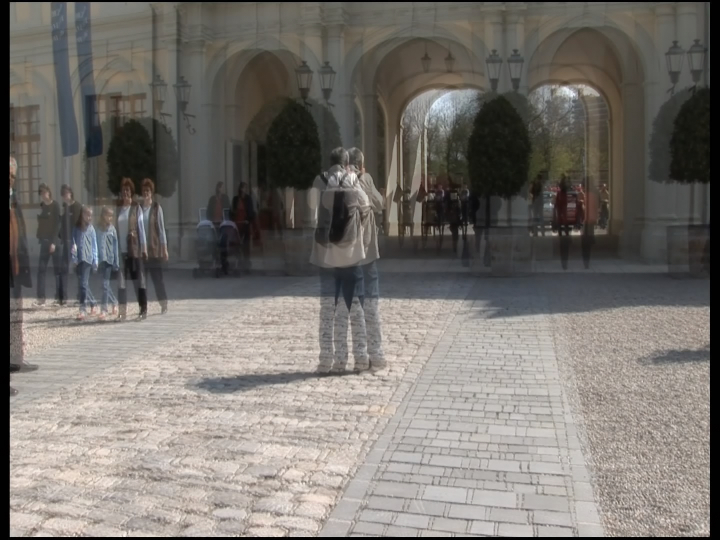
\includegraphics[width=0.6\textwidth]{staticDualView.pdf}
\caption{渲染后输出的3D图像}
\label{fig:staticdualview}
\end{center}
\end{figure}


\subsection{动态3D图像序列的显示}
\label{subsec:motion3dimgdisp}



\section{播放器测试}
\label{sec:3dplayerdemo}

%功能

%瓶颈
